\setAuthor{Päivo Simson}
\setRound{piirkonnavoor}
\setYear{2024}
\setNumber{G 6}
\setDifficulty{6}
\setTopic{TODO}

\prob{Mitteelastne nöör}
\begin{wrapfigure}{r}{0.33\textwidth}
\vspace{-20pt}
  \begin{center}
    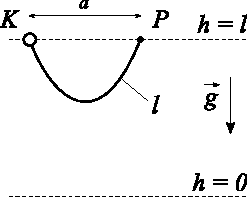
\includegraphics[width=1\linewidth]{2024-v2g-06-yl.pdf}
  \end{center}
  \vspace{-15pt}
\end{wrapfigure}

Väike kuulike on kinnitatud mitteelastse nööri külge ja seda hoitakse esialgu punktis $K$. Nööri pikkus on $l$ ja selle teine ots on kinnitatud punkti $P$. Punktid $K$ ja $P$ asuvad samal kõrgusel $h=l$ ja nendevaheline kaugus on $a$ ($0<a<l$). Nüüd lastakse kuulike ilma algkiiruseta vabaks ja see hakkab gravitatsiooni mõjul liikuma. Leidke maksimaalne kõrgus, mille kuulike saavutab $h=0$ suhtes edaspidise liikumise käigus (pärast täielikku kukkumist). Tehke kuuli trajektoori joonis. Nööri mass on võrreldes kuuli massiga tühine ning takistusjõududega võib mitte arvestada. Nööri mitteelastsus tähendab seda, et põrke hetkel summutab nöör kogu palli nöörisihilise impulsi.


\hint

\solu
\begin{wrapfigure}{r}{0.5\textwidth}
  \vspace{-1em}
  \begin{center}
    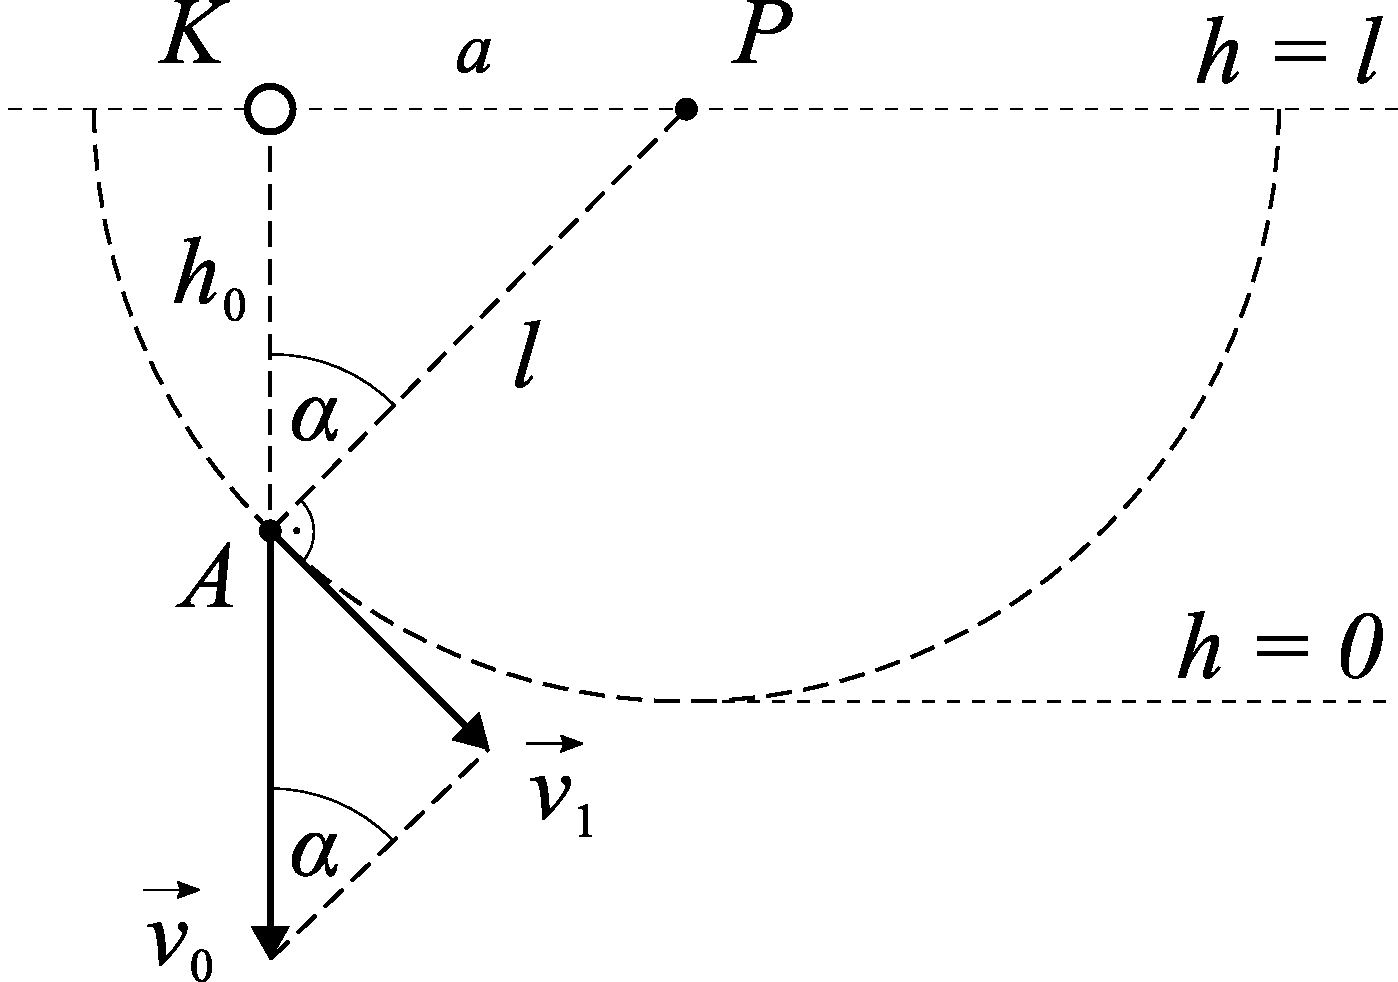
\includegraphics[width=1\linewidth]{2024-v2g-06-sol1.pdf}
  \end{center}
  \vspace{-1em}
\end{wrapfigure}

Kuulike langeb kõigepealt vabalt kõrguse $h_0=\sqrt{l^2-a^2}$ võrra ja saavutab punktis $A$ kiiruse $v_0=\sqrt{2gh_0}$. Selleks hetkeks on nöör sirge ja toimub löök, mille korral tagasipõrget ei toimu, sest nöör on mitteelastne. Löögi käigus kaotab kuulike nöörisihilise kiiruse $\Vec{v}_0$ komponendi ja seega ka osa energiast (kaotatud energia läheb nöörile, mis selle arvelt soeneb). Kuulike jätkab liikumist mööda pikkusega $l$ määratud ringjoone kaart. Säilib ainult kiiruse komponent $v_1$, mis on paralleelne ringjoone puutujaga punktis A: $v_1=v_0\sin\alpha=v_0a/l=\sqrt{2gh_0}\,a/l$. Seega on kuulikese koguenergia vahetult pärast punkti A jõudmist
\[E = \frac{mv_1^2}{2}+mg(l-h_0)=mgh_0\frac{a^2}{l^2}+mg(l-h_0)=\]
\[=mgl\left(1-\frac{h_0}{l}\left(1-\frac{a^2}{l^2}\right)\right)=mgl\left(1-\left(1-\frac{a^2}{l^2}\right)^{\frac{3}{2}}\right).\]
Vabalangemisele järgnevalt jääb kuulike mööda ringjoone kaart võnkuma. Trajektoori kõrgeimas punktis on kuulikese kiirus null ja koguenergia on järelikult $E=mgH$, kus $H$ on otsitav maksimaalne kõrgus. Võrdsustades koguenergia avaldised saame
\[H=l\left(1-\left(1-\frac{a^2}{l^2}\right)^{\frac{3}{2}}\right).\]

\begin{wrapfigure}{r}{0.5\textwidth}
\vspace{-1cm}
  \begin{center}
    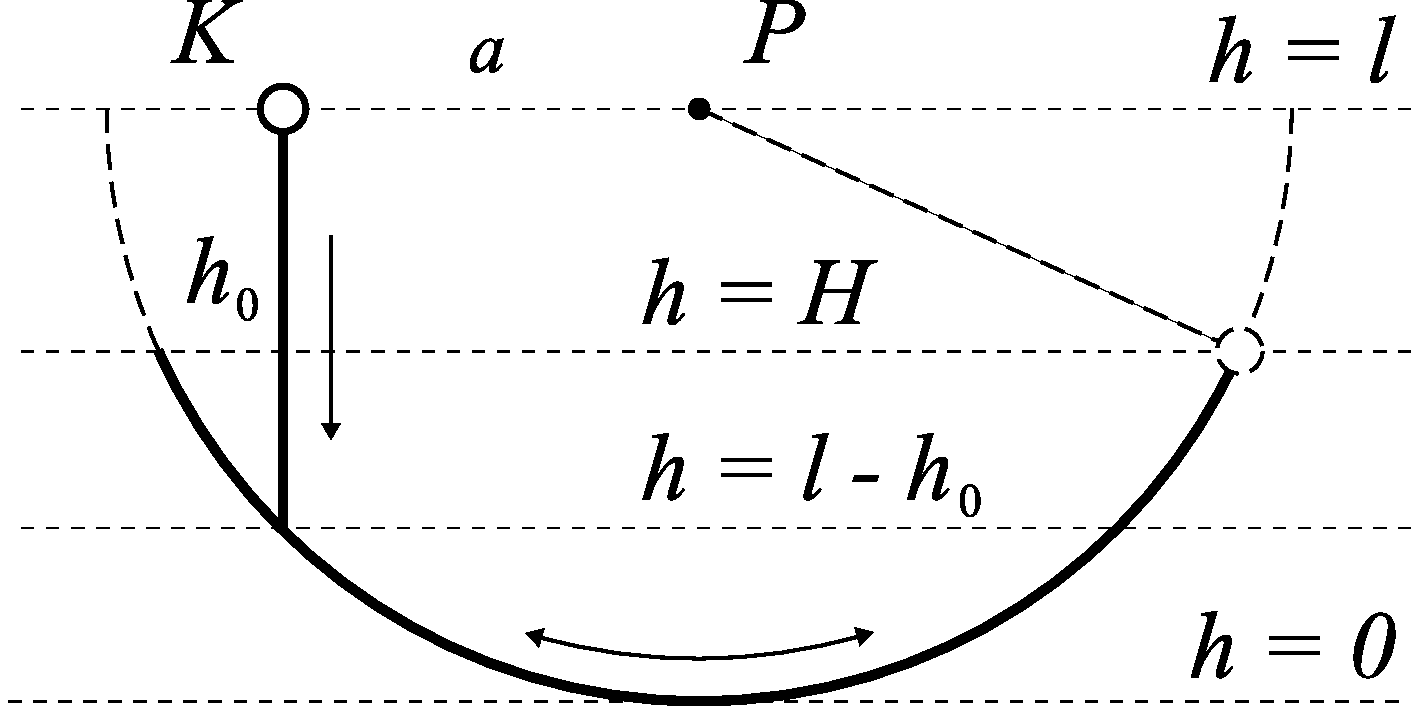
\includegraphics[width=1\linewidth]{2024-v2g-06-sol2.pdf}
  \end{center}
  \vspace{-1.0cm}
\end{wrapfigure}

Trajektoori joonestamiseks võrdleme kõrgusi $H$ ja $l-h_0$. Et $1-a^2/l^2=h_0^2/l^2$ ja $h_0/l<1$, siis
$l(1-h_0^3/l^3)>l(1-h_0/l)$
ehk $H>l-h_0$.
Kuuli trajektoor on näidatud parempoolsel joonisel paksu pideva joonega. Võrratuse $H>l-h_0$ näitamiseks piisab ka tähelepanekust, et punktis $A$, pärast löögi toimumist, on pallil endiselt kineetiline energia olemas ja seega ei saa punkt $A$ olla edasise liikumise kõrgeim punkt.
\probend